%\documentclass[a4paper,pdf]{article} % gebruik acm style voor je scriptie: [format=acmsmall, screen=true, review=false]{acmart} 
%### ACM template on overleaf

%* You can find the ACM template also on overleaf. You can then use the points below for the content.
%* <https://www.overleaf.com/latex/templates/acm-conference-proceedings-master-template/pnrfvrrdbfw>


%\documentclass[sigconf]{acmart} 
\documentclass[sigconf,format=acmsmall, screen=true, review=false]{acmart} 
\usepackage{amsmath}
\usepackage{amsfonts}
\usepackage{amssymb}
\usepackage{hyperref}
\usepackage{pdfpages} % http://mirror.unl.edu/ctan/macros/latex/contrib/pdfpages/pdfpages.pdf
\usepackage{booktabs} 


\usepackage[utf8]{inputenc}
\usepackage{graphicx}
\usepackage[colorinlistoftodos]{todonotes} % handig voor commentaar: gebruik \todo{}, zie ftp://ftp.fu-berlin.de/tex/CTAN/macros/latex/contrib/todonotes/todonotes.pdf
\usepackage{listings}
 
\usepackage{tcolorbox}
\usepackage{float}
\usepackage{caption}
\usepackage{subcaption}


% when writing in Dutch
%\usepackage[dutch]{babel}
%\selectlanguage{dutch}


% linenumbering  See https://texblog.org/2012/02/08/adding-line-numbers-to-documents/
\usepackage{lineno}
\linenumbers

\newcommand{\shorttitle}{} % Put your short title here
\begin{document}




%\input{titlepage}

\begin{titlepage}


\begin{center}
 
\textsc{\Large   The impact of hierarchical social circles on opinion dynamics}

\bigskip

\textsc{\large
submitted in partial fulfillment for the degree of master of science\\
%
\bigskip
Emy B. M. Bakker\\
%
13270176\\
%
\bigskip
master information studies\\
%
data science \\
%
faculty of science\\
%
university of Amsterdam\\
%
\bigskip
Your Date of defence in the format YYYY-MM-DD
}

\end{center}
 
\vfill

\begin{center}
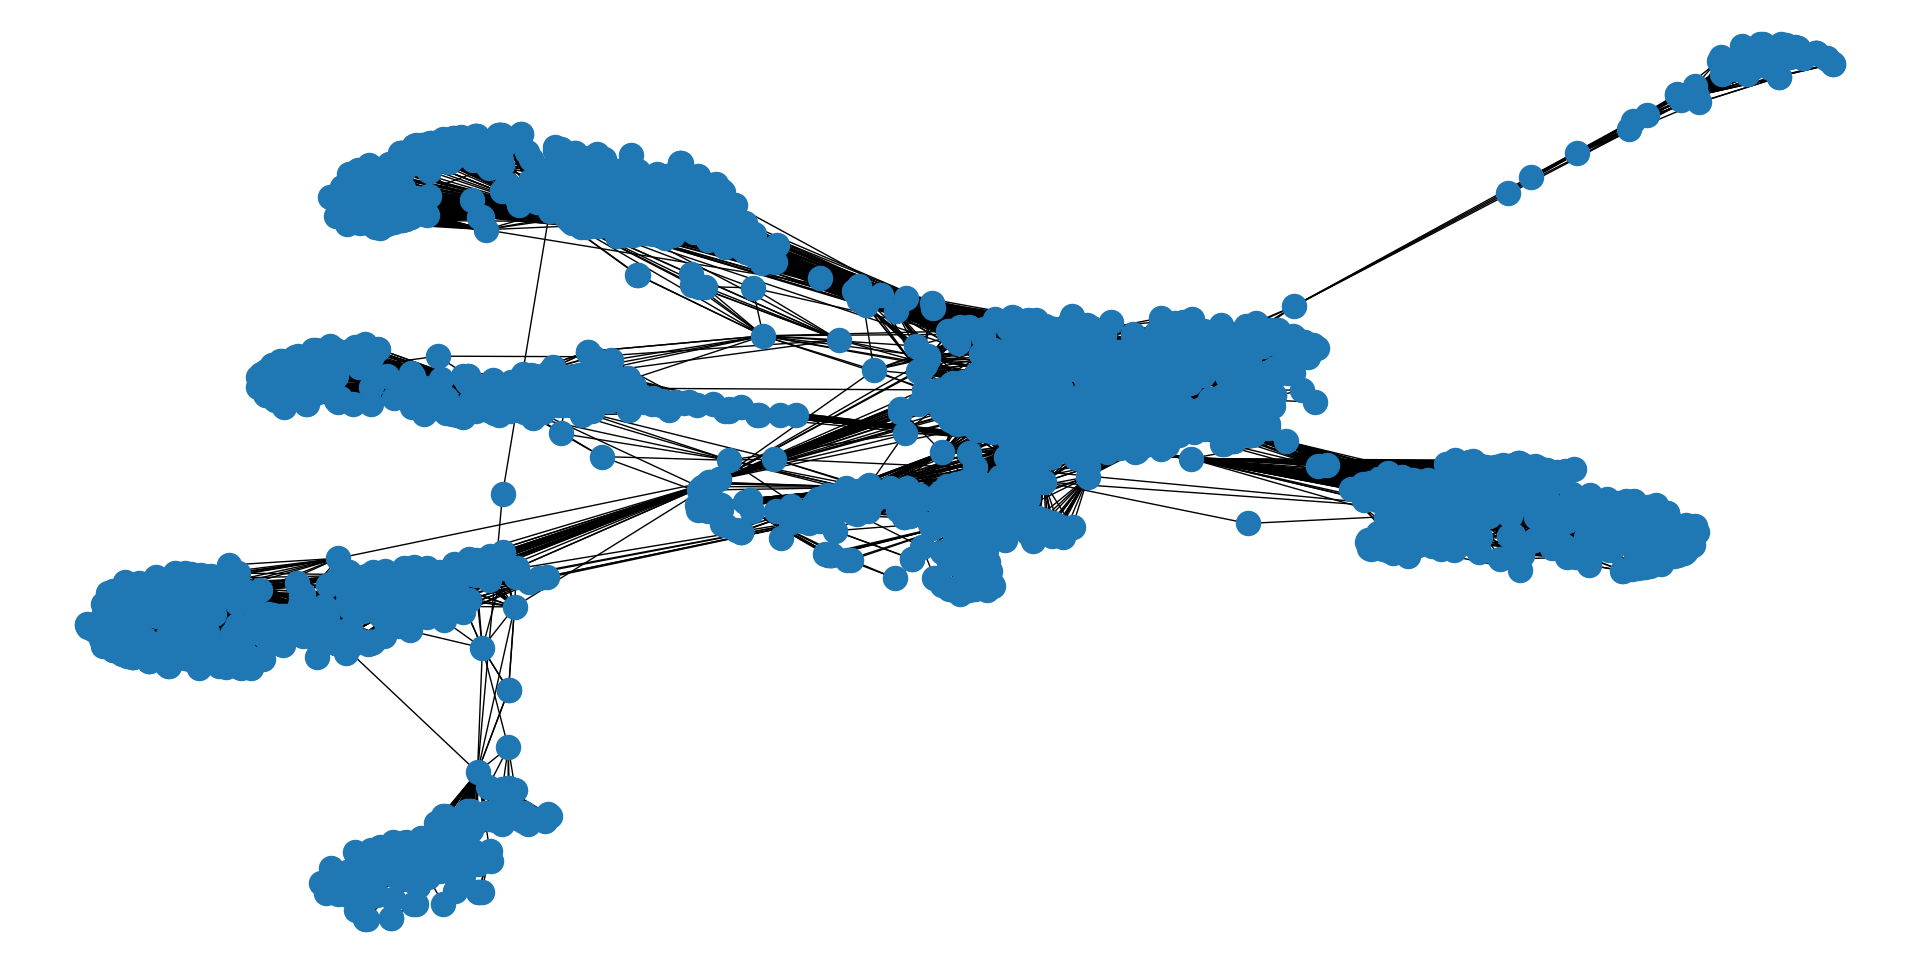
\includegraphics[height=.4\textheight]{Style/TitlePages/logos/Facebook_network.png} %width=\linewidth
\end{center}

\vfill

% In case of an internal project, remove External Supervisor or if you had two internal supervisors, change the header into 
%  & First Supervisor & Second Supervisor  \\
\begin{center}
\begin{tabular}{|l||ll|}
\hline
 & \textbf{Supervisor} & \textbf{Examiner}  \\   
 \hline
\textbf{Title, Name} & Fernando Pascoal Dos Santos & Dr. Maarten Marx\\
\textbf{Affiliation} & UvA & UvA\\ 
\textbf{Email} & f.p.pascoaldossantos@uva.nl & m.j.marx@uva.nl \\
\hline
\end{tabular}
\end{center}

\bigskip
\bigskip
% logos
\begin{center}
\mbox{
\includegraphics[width=.2\paperwidth]{Style/TitlePages/logos/logo-uva.png} 
%
%
\includegraphics[width=.2\paperwidth]{Style/TitlePages/logos/ads.png}
%
\includegraphics[width=.2\paperwidth]{TitlePages/logos/ads.png} % replace by the logo of your internship company or remove
}
\end{center}
\end{titlepage}

%
%\newpage
%
%\end{document}
  % or use another template

\pagebreak

%\todototoc
%\listoftodos
%\tableofcontents

\pagebreak

\begin{abstract}
% [CHANGE] 
\end{abstract}


\section*{Thesis requirements}
\begin{itemize}
\item Your thesis is written in ACM style with two columns  (\texttt{documentclass[sigconf]{acmart}}).
\item   The	size	 of	a	18	EC master	thesis	is	set	at	10	pages	according	to	the	standards	used	for	ACM	and	IEEE	 conferences	 including	 the	 bibliography and	 acknowledgements,	 but excluding	 the	 cover	 page and	appendices.
\item Use one of the conference proceedings available from \url{https://www.acm.org/publications/proceedings-template}
\item Most proceedings authors (including ICPS authors) will use the "sigconf" proceedings template.
\item Use the template at \url{https://github.com/maartenmarx/ThesisTemplate/blob/master/ThesisTemplate/TitlePages/Thesis-Title-Page-DS.tex} for your titlepage.
\end{itemize}


\pagebreak


% Here you input all your sections in seperate files

\input{introduction}
\input{related_work}
\input{methodology}
\input{evaluation}
\input{conclusions}

% your refs

\bibliographystyle{plain}
\bibliography{MyThesis}

\appendix

%\input{appendix}


\section{Slides}

% Example
\includepdf[nup=2x3 , pages=-]{sargent-lecture_slides.pdf}
 
\end{document}
